\documentclass{article}

\usepackage{amsthm}
\usepackage{amsfonts}
\usepackage{amsmath}
\usepackage{amssymb}
\usepackage{fullpage}
\usepackage{graphicx}
\usepackage[usenames]{color}
\usepackage{hyperref}
\usepackage{graphicx}
\usepackage{stmaryrd}
\usepackage{float}
\usepackage{amsmath}




  \hypersetup{
    colorlinks = true,
    urlcolor = blue,       
    linkcolor= blue,      
    citecolor= blue,      
    filecolor= blue,     
    }
    
\usepackage{listings}

\definecolor{dkgreen}{rgb}{0,0.6,0}
\definecolor{gray}{rgb}{0.5,0.5,0.5}
\definecolor{mauve}{rgb}{0.58,0,0.82}

\lstset{frame=tb,
  language=haskell,
  aboveskip=3mm,
  belowskip=3mm,
  showstringspaces=false,
  columns=flexible,
  basicstyle={\small\ttfamily},
  numbers=none,
  numberstyle=\tiny\color{gray},
  keywordstyle=\color{blue},
  commentstyle=\color{dkgreen},
  stringstyle=\color{mauve},
  breaklines=true,
  breakatwhitespace=true,
  tabsize=3
}

\theoremstyle{plain} 
   \newtheorem{theorem}{Theorem}[section]
   \newtheorem{corollary}[theorem]{Corollary}
   \newtheorem{lemma}[theorem]{Lemma}
   \newtheorem{proposition}[theorem]{Proposition}
\theoremstyle{definition}
   \newtheorem{definition}[theorem]{Definition}
   \newtheorem{example}[theorem]{Example}
\theoremstyle{remark}    
  \newtheorem{remark}[theorem]{Remark}

\title{CPSC 354 Report}
\author{Andrew Eppich  \\ Chapman University}
\date{\today}

\begin{document}

\maketitle

\begin{abstract}

\end{abstract}

\tableofcontents

\section{Introduction}\label{intro}

\section{Homework 1}\label{homework1}

\subsection{Question 5}

\begin{lstlisting}
rw [add_zero]
rw [add_zero]
rfl
\end{lstlisting}

\subsubsection{Proof Explanation}

For this question, the Lean proof is related to the corresponding proof in mathematics because we know that we can use the additive identity property, which says that \(x + 0 = x\). By using this, we can simplify \(b + 0\) and \(c + 0\) easily to get \(a + b + c = a + b + c\), which we can determine is the same by the reflexivity property, which states that if \(a = b\), then \(a\) and \(b\) are identical. Therefore, \(a + b + c\) is identical to \(a + b + c\).

\subsection{Question 6}

\begin{lstlisting}
rw [add_zero c]
rw [add_zero b]
rfl
\end{lstlisting}


\subsection{Question 7}

\begin{lstlisting}
rw [one_eq_succ_zero]
rw [add_succ]
rw [add_zero]
rfl
\end{lstlisting}


\subsection{Question 8}

\begin{lstlisting}
rw [two_eq_succ_one]
rw [one_eq_succ_zero]
rw [add_succ]
rw[add_succ]
rw [add_zero]
rw [four_eq_succ_three]
rw [three_eq_succ_two]
rw [two_eq_succ_one]
rw [one_eq_succ_zero]
rfl
\end{lstlisting}

\subsection{Discord Question}

I was wondering if the computers use of discrete math extends to all program computations or just math computations

\section{Homework 2}\label{homework2}

\subsection{Question 1}

\begin{lstlisting}
induction n with d hd
rw [add_zero]
rfl
rw [add_succ]
rw [hd]
rfl
\end{lstlisting}

\subsection{Question 2}

\begin{lstlisting}
  induction b with d hd
  rw [add_zero]
  rw [add_zero]
  rfl
  rw [add_succ]
  rw [add_succ]
  rw [hd]
  rfl
\end{lstlisting}

\subsection{Question 3}

\begin{lstlisting}
induction b with d hd
rw [add_zero]
rw [zero_add]
rfl
rw [add_succ]
rw [hd]
rw [succ_add]
rfl
\end{lstlisting}

\subsection{Question 4}

\begin{lstlisting}
  induction a with d hd
  rw [zero_add]
  rw [zero_add]
  rfl
  rw [succ_add]
  rw [succ_add]
  rw [succ_add]
  rw [hd]
  rfl
\end{lstlisting}

\subsubsection{Explaination}

The lean proof relates to the proof in mathematics because it uses induction to solve the problem. Then the Lean proof is solved by solving the equation of the successors. Just like in mathematics it uses simple rules to change the positioning of the parenthesis so each side is exactly the same. This is exactly like how the mathematical proof would be written.

\subsection{Question 5}

\begin{lstlisting}
  induction a with d hd
  rw [zero_add]
  rw [zero_add]
  rw [add_comm]
  rfl
  rw [add_comm]
  rw [add_comm]
  rw [succ_add]
  rw [succ_add]
  rw [succ_add]
  rw [succ_add]
  rw [hd]
  rfl
\end{lstlisting}

\subsection{Discord Question}

I was wondering how discrete math and the recursive algorithms we talked about fit into a programming language and how it actually works

\section{Homework 3}\label{homework3}

\subsection{Discord Post}

Discord Name: Andrew Eppich.   
In my literature review with ChatGPT, I explored interpreted vs. compiled programming languages. I found that interpreted languages are changed from user to machine code line by line, which is inefficient. Compiled languages are compiled from user to machine code all at once and then run which makes it faster and easier to spot errors. From there I explored interpreted languages and their role in machine learning as well as their history in machine learning. I first found that compiled was much more efficient than interpreted. I then found out that interpreted is mainly used for machine learning. It is mainly used because of the extensive amount of libraries used with interpreted languages, especially Python. Some of those libraries include NumPy, pandas, scikit-learn, TensorFlow, and Matplotlib. These libraries are crucial for machine learning because they are associated with data processing and deep learning. I then took a look into the history of programming languages with machine learning. I found that at first compiled languages were used from the 1950s-1980s. In 1991, Python was developed which became the standard for machine learning in the early 2000s. Python became the main language for machine learning from 2010 and on because of its libraries TensorFlow and PyTorch. 
\url{https://github.com/AndrewEppich/LLM-Literature-Review/blob/main/README.md}

\subsection{Reports Voted For}

\url{https://github.com/zackklopukh/LLMReport}

\url{https://github.com/maxler0y/354_HW3}

\section{Homework 4}\label{homework4}

\begin{figure}[H]
  \centering
  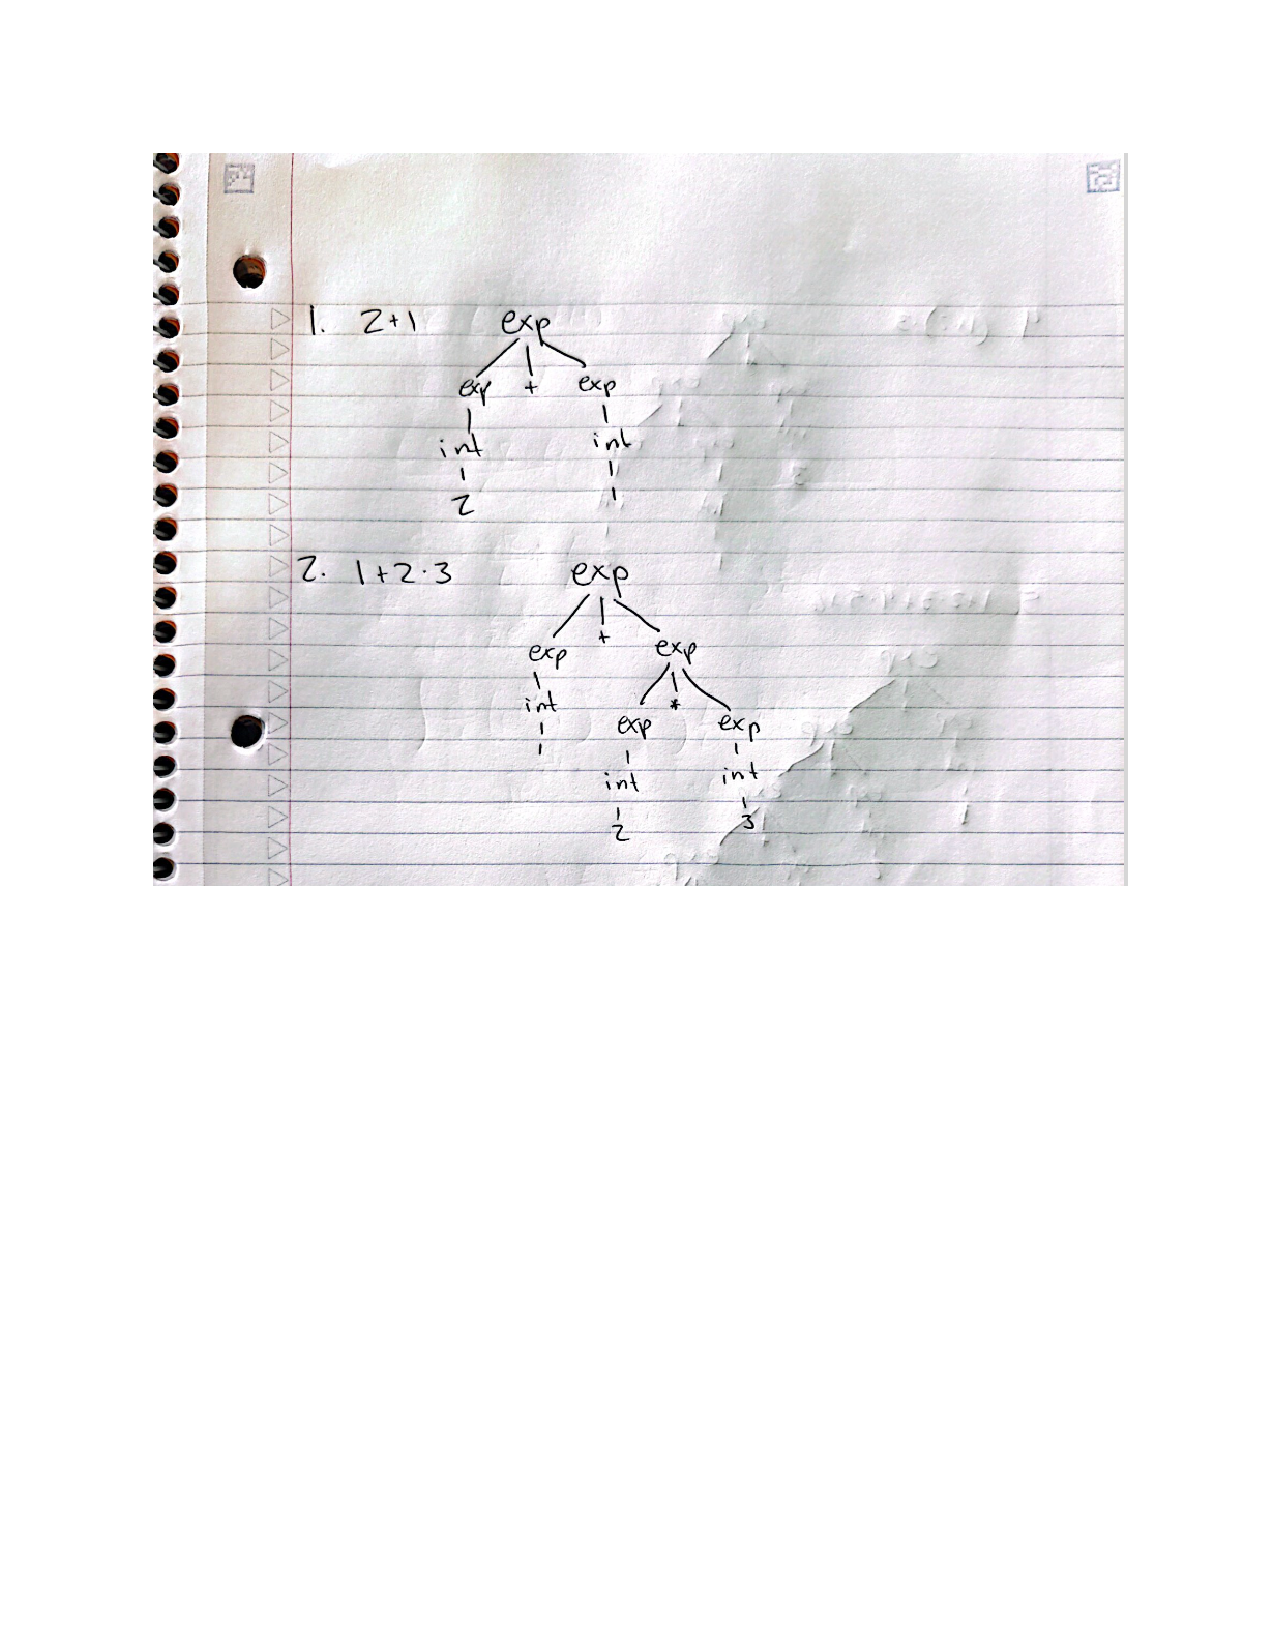
\includegraphics[width=0.7\textwidth, page=1]{Homework_4_trees.pdf}
  \caption{Homework 4 - Page 1}
  \label{fig:homework4_page1}
\end{figure}

\begin{figure}[H]
  \centering
  \includegraphics[width=0.7\textwidth, page=2]{Homework_4_trees.pdf}
  \caption{Homework 4 - Page 2}
  \label{fig:homework4_page2}
\end{figure}

\begin{figure}[H]
  \centering
  \includegraphics[width=0.7\textwidth, page=3]{Homework_4_trees.pdf}
  \caption{Homework 4 - Page 3}
  \label{fig:homework4_page3}
\end{figure}

\begin{figure}[H]
  \centering
  \includegraphics[width=0.7\textwidth, page=4]{Homework_4_trees.pdf}
  \caption{Homework 4 - Page 4}
  \label{fig:homework4_page4}
\end{figure}

\subsection{Discord Question}

How complex do parsing algorithms get the farther down the level of programming languages you go?


\section{Homework 5}\label{homework5}

\subsection{Question 1}

\begin{lstlisting}
  exact todo_list
\end{lstlisting}

\subsection{Question 2}

\begin{lstlisting}
  exact and_intro p s
\end{lstlisting}

\subsection{Question 3}

\begin{lstlisting}
  exact <a,i>, <o,u>
\end{lstlisting}

\subsection{Question 4}

\begin{lstlisting}
  have p := vm.left
  exact p
\end{lstlisting}

\subsection{Question 5}

\begin{lstlisting}
  exact and_right h
\end{lstlisting}

\subsection{Question 6}

\begin{lstlisting}
  have a:= and_left h1
  have b := and_right h2
  exact < a, b>
\end{lstlisting}

\subsection{Question 7}

\begin{lstlisting}
  have h1 := h.right
  have h2 := h.left
  have h3 := h2.right
  exact h.left.right.left.left.right
\end{lstlisting}

\subsection{Question 8}

\begin{lstlisting}
  have h1 := and_left h
  have h2 := and_right h
  have h3 := and_right h2
  have h4 := and_left h3
  have h5 := and_left h4
  have h6 := and_right h1
  have h7 := and_left h1
  have h8 := and_left h7
  have h9 := and_right h7
  exact < h6, h5, h8, h9>
\end{lstlisting}

\subsubsection{Proof Explaination}
I took the left and right sides and set them equal to different variables. Next I took those broken down parts and continued to break them down into different variables until I had a single value for a single variable. Then I added the desired variables together to acheive the desired equation

\subsection{Discord Question}
When thinking about the final Lean problem on the homework, I solved it by breaking up each term over and over again with and\_left and and\_right until there were single terms. It was like a tree forming a new branch and leaves every time the equation was broken up. My question is, how is the logic of AND and and\_left and and\_right used in programming languages and other applications? And is this just the logic that is used to parse a BST?	

\section{Homework 6}\label{homework6}

\subsection{Lecture Explaination}

\begin{lstlisting}
  In class this week we learned about proofs in natural deduction. We talked about the proof of A conjunction B -> C then A -> (B -> C) and also the theorem A -> (B -> C) then (A conjunction B) -> C. we also began talking about lambda calculus. First we talked about lambda abstraction with \x. e which is abstraction because the function does not depend on x anymore. We also learned the abstract syntax of lambda calculus. Also we learned rules of dropping parenthesis in lambda calculus like application associates to the left and appl;ication has a higher precedence than abstraction
\end{lstlisting}

\subsection{Question 1}

\begin{lstlisting}
exact bakery_service p
\end{lstlisting}

\subsection{Question 2}

\begin{lstlisting}
  have h1 : C -> C := fun C \mapsto C
  exact h1
  \end{lstlisting}
  
  \subsection{Question 3}
  
  \begin{lstlisting}
    exact fun h : I \mapsto and_intro (and_right h) h.left
    \end{lstlisting}


\subsection{Question 4}

\begin{lstlisting}
exact fun c => h2 (h1 c)
\end{lstlisting}

\subsection{Question 5}

\begin{lstlisting}
have q : Q := h1 p
have t : T := h3 q
exact h5 t
\end{lstlisting}

\subsection{Question 6}

\begin{lstlisting}
exact fun c => fun d => h <c, d>
\end{lstlisting}

\subsection{Question 7}

\begin{lstlisting}
exact fun h1 => h h1.1 h1.2
\end{lstlisting}

\subsection{Question 8}

\begin{lstlisting}
exact fun s => < h.1 s, h.2 s>
\end{lstlisting}

\subsection{Question 9}

\begin{lstlisting}
exact fun r => < fun s => r, fun ns => r>
\end{lstlisting}

\subsection{Discord Question}

are lambda calculus proofs a part of the compiler? if so, how do they interact with the code that is being compiled?


\section{Homework 7}\label{homework7}

\subsection{Question 1}

\begin{align*}
  & (\lambda m.\lambda n.m \, n)(\lambda f.\lambda x.f(fx))(\lambda f.\lambda x.f(f(fx))) \\
  & \overset{\beta}{\to} (\lambda n.(\lambda f.\lambda x.f(fx))n)(\lambda f.\lambda x.f(f(fx))) \\
  & \overset{\beta}{\to} (\lambda f.\lambda x.f(fx))(\lambda f.\lambda x.f(f(fx))) \\
  & \overset{\beta}{\to} \lambda x.(\lambda f.\lambda x.f(f(fx)))((\lambda f.\lambda x.f(f(fx)))x) \\
  & \overset{\beta}{\to} \lambda x.\lambda x_1.(\lambda f.\lambda x.f(f(fx)))x((\lambda f.\lambda x.f(f(fx)))x((\lambda f.\lambda x.f(f(fx)))x \, x_1)) \\
  & \overset{\beta}{\to} \lambda x.\lambda x_1.(\lambda x_1.x(x(xx_1)))((\lambda f.\lambda x.f(f(fx)))x((\lambda f.\lambda x.f(f(fx)))x \, x_1)) \\
  & \overset{\beta}{\to} \lambda x.\lambda x_1.x(x(x((\lambda f.\lambda x.f(f(fx)))x((\lambda f.\lambda x.f(f(fx)))x \, x_1)))) \\
  & \overset{\beta}{\to} \lambda x.\lambda x_1.x(x(x((\lambda x_1.x(x(xx_1)))((\lambda f.\lambda x.f(f(fx)))x \, x_1)))) \\
  & \overset{\beta}{\to} \lambda x.\lambda x_1.x(x(x(x(x(x((\lambda f.\lambda x.f(f(fx)))x \, x_1)))))) \\
  & \overset{\beta}{\to} \lambda x.\lambda x_1.x(x(x(x(x(x((\lambda x_1.x(x(xx_1)))x_1)))))) \\
  & \overset{\beta}{\to} \lambda x.\lambda x_1.x(x(x(x(x(x(x(x(xx_1)))))))).
\end{align*}


\subsection{Question 2}

The function takes two Church numerals m and n and applies m to n. Applying m to n implements exponentiation where m is the exponent and n is the base

\subsection{Discord Questions}

how complex does lambda calculus recursion get in computer systems?


\section{Homework 8-9}\label{homework89}

\subsection{Question 2}

  a b c d reduces to that because in the code it parses the expression and characterizes it as app which is in the lark grammar defined as exp1 exp2 so it takes a and b and puts parenthesis around it. Then it goes to the next expression whcih is /(a + b /) and then gets the next term which is c so it puts parenthesis around /(a + b /) and c. Then it does this process again with d. then if you have /(a/) it will just return a because in lark grammar it is characterized as var. In the code if the expression is var it returns just the term in the parenthesis so it just returns a

\subsection{Question 3}

Capture avoiding subsittuion works because when when substituting variables, if there is a free variable in the expression then substituting variables in the equation can cause the expression to change its meaning. Capture-avoiding substitutions avoid capturing free variables in the expression when changing a variable which can cause the whole expression to change its meaning. in the code it checks bound variable matches the substitution target, if it does it leaves it unchanged if not it generates a new variable

\subsection{Question 4}

We do not always get the expected results. Well-defined expressions typically return the expected results, but if there is an error handling an edge case, it would not return the expected results. Not all computations reduce to normal form. Expressions like \((\lambda x. \, x \, x)\) and \((\lambda x. \, x \, x)\) create an infinite loop of self-application that will never be stable.

\subsection{Question 5}

This is the smallest lambda function that doesn’t reduce to normal form: \((\lambda x. \, x \, x) \, (\lambda x. \, x \, x)\). This reduces to itself, so there is no normal form.

\subsection{Quesdtion 7}

\textbf{Initial Expression}:
\[
((\lambda m.\, \lambda n.\, m \, n) \, (\lambda f.\, \lambda x.\, f \, (f \, x))) \, (\lambda f.\, \lambda x.\, f \, (f \, (f \, x)))
\]

\textbf{First Application}:
Apply \((\lambda m.\, \lambda n.\, m \, n)\) to \((\lambda f.\, \lambda x.\, f \, (f \, x))\):
\[
(\lambda n.\, (\lambda f.\, \lambda x.\, f \, (f \, x)) \, n)
\]

\textbf{Second Application}:
Now apply \((\lambda n.\, (\lambda f.\, \lambda x.\, f \, (f \, x)) \, n)\) to \((\lambda f.\, \lambda x.\, f \, (f \, (f \, x)))\), substituting \(n\) with \((\lambda f.\, \lambda x.\, f \, (f \, (f \, x)))\):
\[
(\lambda f.\, \lambda x.\, f \, (f \, x)) \, (\lambda f.\, \lambda x.\, f \, (f \, (f \, x)))
\]

\textbf{Evaluating the Final Application}:
Substitute \((\lambda f.\, \lambda x.\, f \, (f \, (f \, x)))\) for \(f\) in \((\lambda f.\, \lambda x.\, f \, (f \, x))\):
\[
\lambda x.\, ((\lambda f.\, \lambda x.\, f \, (f \, (f \, x))) \, x)
\]

\textbf{Result}:
The final expression (in normal form) is:
\[
\lambda x.\, (\lambda f.\, \lambda x.\, f \, (f \, (f \, x))) \, x
\]

\subsection{Question 8}

\begin{verbatim}
  12: evaluate(((\m.\n. m n) (\f.\x. f (f x))) (\f.\x. f x))
      39: evaluate((\m.\n. m n) (\f.\x. f (f x)))
          12: evaluate(\m.\n. m n) = \m.\n. m n
          12: evaluate(\f.\x. f (f x)) = \f.\x. f (f x)
          51: substitute(\n. m n, m, (\f.\x. f (f x)))
              51: substitute((\f.\x. f (f x)) n, n, (\f.\x. f x))
          12: evaluate((\n. (\f.\x. f (f x)) n))
              51: substitute((\f.\x. f (f x)) n, n, (\f.\x. f x))
      39: evaluate((\f.\x. f (f x)) (\f.\x. f x))
          51: substitute((\x. f (f x)), f, (\f.\x. f x))
              51: substitute((\x. ((\f.\x. f x) ((\f.\x. f x) x))), f, (\f.\x. f x))
  \end{verbatim}

\subsection{Discord Questions}

Week 8: What does it mean in terms of a programming language output when something does not reduce to normal form

Week 9: how often is tracing used in the debugger in industry


\section{Homework 10}\label{homework10}

1. I found that figuring out the debugger and how to use the print statements like print(linearize(x)) was the hardest aspect because it took a while for me to get it to work

2. I came up with the key insight because I was struggling to figure out how to make sure the MWE returned the correct result. I figured out that if the expressions were identical then the result would be the same as the expressions. So i added a part that checked for that

3. The most interesting takeaway from this was learning how to use code to evaluate the lambda expressions

\subsection{Discord Question}

week 10: what aspects if coding prompts substitutions to be made to evaluate it

\section{Homework 11}\label{homework11}

\begin{figure}[H]
  \centering
  \includegraphics[width=0.7\textwidth, page=1]{HW11.pdf}
  \caption{Homework 11 - Page 1}
  \label{fig:homework11_page1}
\end{figure}

\begin{figure}[H]
  \centering
  \includegraphics[width=0.7\textwidth, page=2]{HW11.pdf}
  \caption{Homework 11 - Page 2}
  \label{fig:homework11_page2}
\end{figure}


\subsection{Discord Question}

If an ARS is not terminating is that a similar situation to when code has an infinite loop


\section{Homework 12}\label{homework12}

\subsection{Exercise 1}

* The ARS terminates because it is reduced to a unique form 
* The result of the computation is ab, which is the sorted version of the original
* It is unique because it is sorted so it can not be reduced anymore
* This algorithm implements bubble sort

\subsection{Exercise 2}

* The ARS terminates because it cannot be reduced any more
* The normal forms are a and b
* There is no string that will reduce to a and b, there have to be an even number of a to reduce to a but there have to be an odd number of b to reduce to a
* It is confluent because all reductions lead to a unique normal form
* If you replace -> with = then aa = bb and ab = ba
* The expression is equal to a when there is an even number of bs and equal to be if there are an odd number of bs
* Even count of bs → a, odd count of bs → b
* The algorithm computes whether there is an odd or even amount of bs

\subsection{Exercise 3}

* The algorithm does not terminate because when ba -> ab and ab -> ba so there is an infinite loop of reduction
* There are no normal forms because it does not terminate
* Change ab → ba to ab → b
* The algorithm removes duplicates from the string

\subsection{Exercise 4}

* The ARS does not terminate because ab → ba and ba → ab makes an infinite loop
* There are no normal forms because it does not terminate
* The results are not confluent because they do not reduce to a unique result
* This algorithm allows a and b to be switched to find all permutations of sequences with ab

\subsection{Exercise 5}

* abba → abba , bababa → bababa
* It is not terminating because ab → ba and ba → ab allow looping
* One class for each combination of counts of as and bs, there are no normal forms
* You can modify ba → ab to ba → b
* One question you can answer using this ARS is if two strings are equivalent 

\subsection{Exercise 5b}

* abba → abba, bababa → bababa
* It does not terminate because ab → ba and ba → ab allow for infinite looping
* The equivalence classes are the count of as modulo 2, and complete removal of bs the 
* Normal forms are both a
* Is the parity of as preserved in the equivalence class

\subsection{Discord Question}

what other uses do ARSs have besides sorting strings and how are they implemented 


\section{Homework 13}\label{homework13}

\[
\text{let rec } \mathit{fact} = \lambda n. \text{ if } n = 0 \text{ then } 1 \text{ else } n \cdot \mathit{fact}(n-1) \text{ in } \mathit{fact}(3)
\]
\[
\to \text{\textbf{<def of let rec>}} \quad \mathit{fact} = \mathit{fix} \, F, \text{ where } F = \lambda f. \lambda n. \text{if } n = 0 \text{ then } 1 \text{ else } n \cdot f(n-1)
\]
\[
\to \mathit{fix} \, F \, 3 \quad \text{\textbf{<def of fix>}}
\]
\[
\to F(\mathit{fix} \, F) \, 3 \quad \text{\textbf{<beta rule: substitute } F\text{>}}
\]
\[
\to (\lambda f. \lambda n. \text{if } n = 0 \text{ then } 1 \text{ else } n \cdot f(n-1))(\mathit{fix} \, F) \, 3
\]
\[
\to \lambda n. \text{if } n = 0 \text{ then } 1 \text{ else } n \cdot (\mathit{fix} \, F)(n-1) \quad \text{\textbf{<beta rule>}}
\]
\[
\to \text{if } 3 = 0 \text{ then } 1 \text{ else } 3 \cdot (\mathit{fix} \, F)(3-1) \quad \text{\textbf{<beta rule: substitute } 3\text{>}}
\]
\[
\to 3 \cdot (\mathit{fix} \, F)(2) \quad \text{\textbf{<def of if>}}
\]
\[
\to 3 \cdot F(\mathit{fix} \, F)(2) \quad \text{\textbf{<def of fix>}}
\]
\[
\to 3 \cdot (\lambda f. \lambda n. \text{if } n = 0 \text{ then } 1 \text{ else } n \cdot f(n-1))(\mathit{fix} \, F)(2) \quad \text{\textbf{<beta rule>}}
\]
\[
\to 3 \cdot (\lambda n. \text{if } n = 0 \text{ then } 1 \text{ else } n \cdot (\mathit{fix} \, F)(n-1))(2) \quad \text{\textbf{<beta rule>}}
\]
\[
\to 3 \cdot (\text{if } 2 = 0 \text{ then } 1 \text{ else } 2 \cdot (\mathit{fix} \, F)(2-1)) \quad \text{\textbf{<beta rule: substitute } 2\text{>}}
\]
\[
\to 3 \cdot (2 \cdot (\mathit{fix} \, F)(1)) \quad \text{\textbf{<def of if>}}
\]
\[
\to 3 \cdot (2 \cdot F(\mathit{fix} \, F)(1)) \quad \text{\textbf{<def of fix>}}
\]
\[
\to 3 \cdot (2 \cdot (\lambda f. \lambda n. \text{if } n = 0 \text{ then } 1 \text{ else } n \cdot f(n-1))(\mathit{fix} \, F)(1)) \quad \text{\textbf{<beta rule>}}
\]
\[
\to 3 \cdot (2 \cdot (\lambda n. \text{if } n = 0 \text{ then } 1 \text{ else } n \cdot (\mathit{fix} \, F)(n-1))(1)) \quad \text{\textbf{<beta rule>}}
\]
\[
\to 3 \cdot (2 \cdot (\text{if } 1 = 0 \text{ then } 1 \text{ else } 1 \cdot (\mathit{fix} \, F)(1-1))) \quad \text{\textbf{<beta rule: substitute } 1\text{>}}
\]
\[
\to 3 \cdot (2 \cdot (1 \cdot (\mathit{fix} \, F)(0))) \quad \text{\textbf{<def of if>}}
\]
\[
\to 3 \cdot (2 \cdot (1 \cdot F(\mathit{fix} \, F)(0))) \quad \text{\textbf{<def of fix>}}
\]
\[
\to 3 \cdot (2 \cdot (1 \cdot (\lambda f. \lambda n. \text{if } n = 0 \text{ then } 1 \text{ else } n \cdot f(n-1))(\mathit{fix} \, F)(0))) \quad \text{\textbf{<beta rule>}}
\]
\[
\to 3 \cdot (2 \cdot (1 \cdot (\lambda n. \text{if } n = 0 \text{ then } 1 \text{ else } n \cdot (\mathit{fix} \, F)(n-1))(0))) \quad \text{\textbf{<beta rule>}}
\]
\[
\to 3 \cdot (2 \cdot (1 \cdot (\text{if } 0 = 0 \text{ then } 1 \text{ else } 0 \cdot (\mathit{fix} \, F)(0-1)))) \quad \text{\textbf{<beta rule: substitute } 0\text{>}}
\]
\[
\to 3 \cdot (2 \cdot (1 \cdot 1)) \quad \text{\textbf{<def of if>}}
\]
\[
\to 3 \cdot (2 \cdot 1) = 3 \cdot 2 = 6 \quad \text{\textbf{<combine results>}}
\]
\[
\text{Final Result: } \mathit{fact}(3) = 6
\]

\subsection{Discord Question}

When using recursion in implementing a programming language, is big O notation just as important for optimizing it as it is for implementing data structures in programming for example

\section{Lessons From Group Assignments and Project}\label{lessonsFromGroupAssignmentsAndProject}


The first project I worked on was Project 3. For this assignment, I didn’t have a group, so I took on the challenge of completing the entire project independently. This project required me to implement a minimum working example into a calculator, along with various lambda functions. It was an incredible experience to code functions that we had been studying in class and to finally see how these abstract concepts could be applied to programming in a practical way. One of the most significant parts of this project was adapting the evaluate method to ensure that it could correctly parse the given lambda expressions. The process involved parsing the expression into a tree structure, which then allowed the rest of the program to evaluate it effectively. This concept was similar to Homework 4, where we practiced drawing parsing trees for simple equations, except the trees in this project were much more complex. Seeing how the theoretical aspect translated into real programming was both very interesting. Additionally, it was interesting to observe how the linearize method played a crucial role in breaking down functions so they could be evaluated correctly. Understanding how this method worked provided me with deeper insights into how parsing and evaluation fit together in the larger picture of implementing a lambda calculus interpreter. This assignment proved incredibly helpful in solidifying what we had learned during lectures about beta reductions and parsing trees, as it offered a hands-on opportunity to apply those principles. 


Moving on to Project 4, Milestone 1, I once again found myself working independently. Having successfully completed Project 3 on my own, I was determined to continue proving to myself that I could tackle these challenges without a group. This milestone required me to add arithmetic operations to the interpreter. Parsing trees were once again critical to my understanding of how these functions were decomposed and processed. By leveraging what I had learned previously, I was able to update the evaluate function to handle these new parsing trees correctly. In addition to updating the program's core functionality, I had to write tests for the test file. This was an interesting experience for me as I had only recently started learning about testing and had never done it in Python before. Writing these tests was not only a great way to reinforce my understanding of the project but also an opportunity to gain practical experience with testing frameworks in Python. The arithmetic operations themselves—such as addition, subtraction, multiplication, and negation—were not overly challenging to incorporate into the program. However, I found it interesting how seemingly simple operations required code that appeared quite complex. To make this work, I added plus, minus, times, and neg to the LambdaCalculusTransformer class, as well as made necessary updates to the evaluate, substitute, and linearize methods. Each of these changes required careful thought and attention to detail to ensure that the operations integrated smoothly into the overall interpreter. 


Next, I worked on Assignment 4, Milestone 2, continuing my streak of completing these assignments independently. This milestone involved adding natural language constructs to the interpreter, a task that pushed my understanding of the project even further. Specifically, I implemented if, then, else, let, letrec, and fix. It was interesting to bring these logical structures to life in the interpreter. Implementing the if-then-else logic we discussed in lecture was also interesting. Seeing how the interpreter could process and execute these commands felt like a significant step toward creating a fully functional programming language. In addition to the logical constructs, I also added equality operators such as ==, <=, >=, and !=. This showed me how the theoretical concepts we discussed in class translated into practical coding tasks. Incorporating these operators reminded me of regular programming, where equality checks are essential for writing if statements. The process of adding these operators was an easy extension of the work we had done previously. Since the grammar for if statements was already in place, I could anticipate how this project would evolve. I figured out that these foundational elements would eventually integrate into a system that could support complex logic. By this point, I could clearly see the connection between our lecture material and the code I was writing. Early in the class, I struggled to imagine how we would go from learning lambda calculus to building a full-fledged programming language. However, working on this milestone helped me bridge that gap. I began to understand how the individual components of the interpreter fit together and how they would ultimately contribute to the functionality of the project. 


Finally, I tackled Assignment 4, Milestone 3, which proved to be the most challenging milestone yet. This project took an incredible amount of time and effort to complete, particularly the sorting functionality at the end. Getting the sorting to work correctly took me at least three full days of debugging and testing. In this milestone, I introduced several new features, including prog, hd, tl, nil, and cons. These additions required me to update the grammar, as well as the evaluate and linearize functions, to handle the parsing and evaluation of these new expressions. Initially, parsing the increasingly complex trees was very difficult. The complexity of the trees required me to apply the logic we had covered in class. After many many hours, I was able to write code that passed all the tests successfully. I also implemented sequencing, which allowed two different expressions to be executed in the same test. This feature brought a new level of sophistication to the interpreter. Additionally, I implemented lists, which brought me even closer to finishing the programming language. Seeing how lists and other constructs could be integrated into a project I built myself was very satisfying. This milestone represented the culmination of everything I had learned in the class. It was amazing to see the individual components, like parsing trees, equality operators, and logical constructs, come together to form a functioning programming language.



\section{Conclusion}\label{conclusion}

I enjoyed this course a lot. At first, I was very skeptical of how math would fit into programming languages. After learning all about lambda calculus, recursion, and various evaluation techniques I believe I can step back and have a clear understanding of how a programming language is created and implemented. It was also cool to have other students ask questions on discord and to have the answer explained. I think that helped me put more real world application to the class in general. Taking a step back, I see how important this class is in the scope of software engineering. The content of this course built the groundwork for quite literally the entire software industry. Without lambda calculus, recursion, and other various evaluation techniques there would be no programming languages for people to code on. It is the very foundation of all coding. It kind of blows my mind that I just completed a course that taught me about the very foundation of all software engineering. I found recursion to be very interesting. I never stopped to think about how it actually worked at the most basic level. It was very interesting to take a step out of the world of technology and advanced programming languages and take a look at the bare bones basics that power them. It was also very interesting to learn about lambda calculus and about how functions actually reduce. It was also very interesting to learn about how lambda calculus implements some arithmetic operations with natural numbers. Some of the examples were addition, subtraction, multiplication, and exponentiation. It changed my perspective on lambda calculus because I thought it was just a reduction without any numbers. I also thought parsing was very interesting because I have heard a lot of people using that term without fully understanding what it meant. I feel confident that I know the term completely and its implications after getting to learn the lowest level concepts of parsing. I personally would suggest adding more real world applications into the course as a supplement to the material. I think those real applications helped me to solidify the concept and really see it in a much better way that helped me understand it. Especially, since a lot of people don't like math much and that is just showing a bunch of proofs with no application to real life. I think that would just allow students to understand the significance of the material and apply it better


\section{References}\label{references}

Koopmans, R. (2019, October 22). "Lambda calculus for mortals." Medium. https://medium.com/@ReganKoopmans/lambda-calculus-for-mortals-691013808f9c

Hacker News. (2014, June 7). "What is the significance of lambda calculus?". Hacker News. https://news.ycombinator.com/item?id=7506409

GeeksforGeeks. (2021, February 13). Introduction to parsing, ambiguity, and parsers (Set 1). GeeksforGeeks. https://www.geeksforgeeks.org/introduction-of-parsing-ambiguity-and-parsers-set-1/

Ray, J. (n.d.). Parsing theory. Loyola Marymount University. https://cs.lmu.edu/~ray/notes/parsingtheory/

Hofmann, M. (n.d.). The Curry-Howard isomorphism. Carnegie Mellon University. https://web2.qatar.cmu.edu/cs/15317/lectures/04-curryhoward.pdf

Sellin, E. (2020, November 25). What exactly is Turing completeness? Medium. https://evinsellin.medium.com/what-exactly-is-turing-completeness-a08cc36b26e2

Software Engineering Stack Exchange. (n.d.). What are invariants, how can they be used, and have you ever used it in your programming? Software Engineering Stack Exchange. https://softwareengineering.stackexchange.com/questions/32727/what-are-invariants-how-can-they-be-used-and-have-you-ever-used-it-in-your-pro



\end{document}
